\section{Multi-Vertical Use Case}
\label{chap:proposal:use-case}

To assess the testbed's suitability for the development and validation of vertical applications in an end-to-end scenario, a Network Application will need to be developed and evaluated in the proposed testbed. This will demonstrate the testbed's capabilities and showcase how its underlying infrastructure and interfaces can be used to deploy and validate applications under the requirements of a specific vertical use case. Section \ref{sota:networkapplications:usecases} highlighted several possible network applications across distinct verticals and scenarios, such as \ac{CAM}, \ac{TL}, and \ac{PPDR}. Given the testbed's goal of catering to multiple vertical industries, the considered \ac{PoC} targets the \ac{PPDR} and Automotive sectors through a vehicle collision detection and notification solution that bridges the two domains.

This use case is motivated by the need to improve the safety of road users in the moments immediately after an accident. Following a vehicle collision, involved and nearby vehicles and pedestrians remain exposed to the hazards of the crash site, increasing the risk of secondary incidents before emergency services arrive. Mitigating this risk requires detecting incidents quickly and immediately alerting those at and approaching the crash site. In this scenario, a computer vision model would analyze a live video stream from fixed roadside cameras to detect collisions and trigger notifications in real time, requiring close integration with the mobile network to automate detection and alerting.

\subsection{Application Interaction Flow}
\label{chap:proposal:use-case:flow}

Figure~\ref{fig:proposal:use-case-validation:flow:overview} illustrates a high-level view of the proposed solution and the interactions between its components. The envisioned system consists of three main elements: (i) a fixed roadside camera, acting as an \acs{UE}, that captures live video and streams it over the \acs{5G} network; (ii) an inference server, deployed at the edge or the cloud, that processes the received streams through an \acs{AI} vehicle collision detection model; and (iii) the actual network application that, through the northbound interfaces of the mobile network, manages the network resources supporting the video stream and alerts nearby road users once a collision is detected. In addition, operator dashboards should provide \acs{PPDR} agents with a real-time overview of the monitored road segment, displaying the live camera feeds alongside the detected collision events so they can inspect the scene and corroborate the outputs produced by the \acs{AI} model. Each event must be georeferenced and represented on an interactive map, together with the real-time positions of nearby road users. This information is also expected to be provided by the network.


\begin{figure}[htbp]
    \centering
    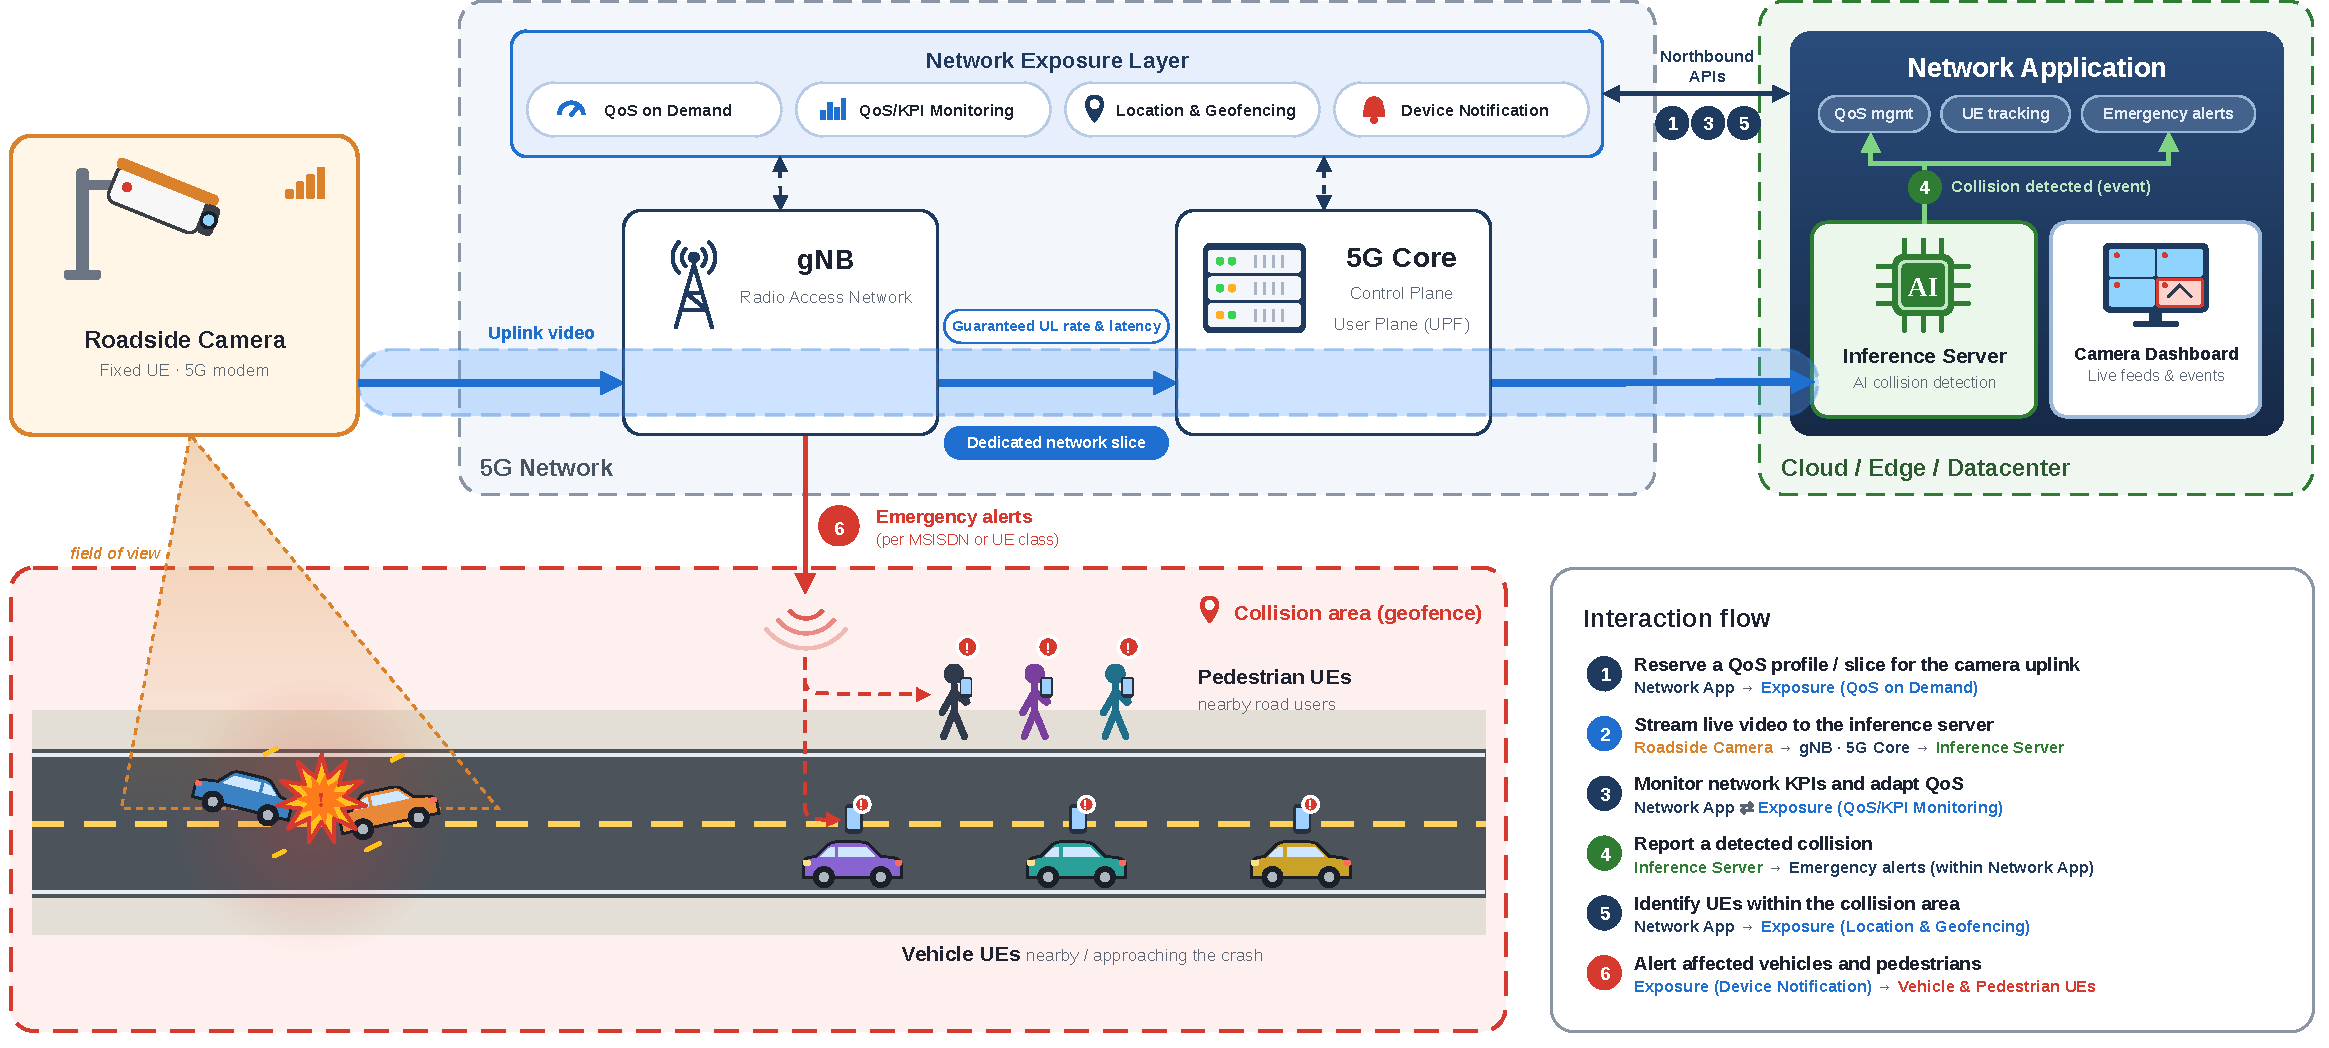
\includegraphics[width=1\linewidth]{figs/drawio/diagrama_napp.pdf}
    \caption{Conceptual overview of the proposed solution}
    \label{fig:proposal:use-case-validation:flow:overview}
\end{figure}



\subsection{Application Requirements}
\label{chap:proposal:use-case:requirements}

With the context and purpose of the network application established, the next step is to derive the requirements for the \acs{PoC} application. These will be organized into two categories: functional and non-functional requirements. Functional requirements describe the system and its functionality, i.e. the tasks it is capable of performing. Non-functional requirements specify the conditions under which the system is required to operate, as well as the properties it must exhibit. This category comprises performance requirements, which define the extent to which the system's functions must be executed through quantitative and individually verifiable metrics, and quality requirements, which capture system criteria such as security and portability.

\subsubsection{Functional Requirements}
\label{chap:proposal:use-case:requirements:functional}

The functional requirements align with the primary functionalities provided by the application. Given the emergency nature of the use case, stakeholders must be able to reserve the network resources needed to support the application. In particular, the uplink connection from the roadside camera to the inference server must satisfy defined throughput and latency requirements to ensure reliable, real-time detection. These requirements should be specified in advance, as part of the application's \acs{QoS} profile, and verified throughout the application's lifecycle. This requires continuous visibility into the network conditions experienced by the application, as the degradation of the communication layer may warrant, for instance, an adjustment of \acs{QoS} to preserve detection performance.

To achieve continuous monitoring and adaptive \acs{QoS}, the application requires exposure interfaces that allow it to interact programmatically with the underlying mobile network and request the necessary network capabilities and \acsp{KPI}. The same applies to other services that are crucial to its operation. The application must identify and track vehicle and pedestrian \acs{UE} within a defined perimeter around the monitored area, to determine which users to alert in case of an emergency. Once a collision is detected, these users must then be notified either individually, e.g. by \acs{MSISDN}, or collectively, by targeting a specific class of \acsp{UE}, such as those associated with pedestrians or vehicles. These capabilities, however, depend on the network infrastructure, and the testbed, exposing the necessary functionality to third-party applications through appropriate interfaces. Accordingly, the functional requirements of the application are defined as follows:

\begin{custenumerate}{FR}
    \item \label{enum:fr:slice} The system shall request, prior to its operation, the reservation of network resources dedicated exclusively to the application, isolated from other traffic sharing the mobile network, according to custom \acs{QoS} connectivity requirements;
    \item \label{enum:fr:stream} The system shall establish a live video stream from the roadside camera to the inference server over the \acs{5G} network;
    \item \label{enum:fr:detection} The system, i.e. the inference server, shall analyze each frame received from the video stream to detect vehicle collisions;
    \item \label{enum:fr:detection-event} The system shall report each detected vehicle collision as an event from the inference server to the network application;
    \item \label{enum:fr:dashboard} The system shall provide \acs{PPDR} agents with an operator dashboard presenting a real-time overview of the monitored road segment, including the live video stream from the roadside camera;
    \item \label{enum:fr:dashboard-collisions} The system shall display each detected vehicle collision on the operator dashboard, georeferenced on an interactive map;
    \item \label{enum:fr:qos-profile} The system shall reference a \acs{QoS} profile for the camera's data session, specifying the uplink throughput and latency to be requested from the network;
    \item \label{enum:fr:monitoring-profile} The system shall define a monitoring profile for the camera's data session, specifying the throughput and latency thresholds against which the observed network conditions should be evaluated;
    \item \label{enum:fr:qos-request} The system shall request the network \acsp{KPI} specified in the referenced \acs{QoS} profile for the camera's data session;
    \item \label{enum:fr:monitoring} The system shall monitor the network conditions experienced by the camera's data session, comparing them against the thresholds defined in the monitoring profile;
    \item \label{enum:fr:qos-change} The system shall change the active \acs{QoS} profile of the camera's data session whenever the monitored network conditions violate the thresholds defined in the monitoring profile;
    \item \label{enum:fr:ue-tracking} The system shall identify and actively track all vehicle and pedestrian \acsp{UE} in the vicinity of the surveilled area, displaying their real-time positions on the operator dashboard;
    \item \label{enum:fr:geofencing} The system shall detect all vehicle and pedestrian \acsp{UE} located within or entering a predefined area around the surveilled area;
    \item \label{enum:fr:notify-pedestrians} The system shall notify all pedestrian \acsp{UE} located within the predefined area identified in \ref{enum:fr:geofencing}, at the moment the collision detection event is processed;
    \item \label{enum:fr:notify-vehicles} The system shall notify all vehicle \acsp{UE} located within the predefined area identified in \ref{enum:fr:geofencing}, at the moment the collision detection event is processed;
    \item \label{enum:fr:notify-periodic} The system shall periodically reissue alert notifications to the appropriate \acsp{UE} until the incident is deemed resolved.
\end{custenumerate}

\subsubsection{Non-Functional Requirements}
\label{chap:proposal:use-case:requirements:nonfunctional}

The non-functional requirements specify the operational constraints that govern the execution of the functionalities defined above. Among these, the performance requirements are presented first, each linked to the functional requirements specified in Section~\ref{chap:proposal:use-case:requirements:functional} whose execution it constrains:

\begin{custenumerate}{NFR}
    \item \label{enum:nfr:uplink-bitrate} The uplink connection between the camera and the inference server shall sustain a guaranteed minimum bitrate sufficient to deliver the video stream at a rate of at least 30 \acs{FPS} (\ref{enum:fr:stream}, \ref{enum:fr:qos-profile}, \ref{enum:fr:qos-request});
    \item \label{enum:nfr:frame-processing} The system, i.e. the inference server, shall process at least one out of every three consecutive frames of the 30 \acs{FPS} input stream, such that no more than two consecutive frames are skipped at any given time (\ref{enum:fr:stream}, \ref{enum:fr:detection});
    \item \label{enum:nfr:degradation-detection} The system shall detect a degradation of the network conditions below the requirements declared in the \acs{QoS} profile within 1 second of its occurrence (\ref{enum:fr:monitoring-profile}, \ref{enum:fr:monitoring});
    \item \label{enum:nfr:qos-enforcement} The system shall enforce the new \acs{QoS} profile within 1 second of the degradation being detected (\ref{enum:fr:qos-change});
    \item \label{enum:nfr:notification-time} The system shall notify the affected \acsp{UE} within 1 second of the collision detection event (\ref{enum:fr:detection-event}, \ref{enum:fr:notify-pedestrians}, \ref{enum:fr:notify-vehicles}).
\end{custenumerate}

It should be noted that the verifiability of some of the performance requirements listed above is not determined exclusively by the envisioned system, but also by the capabilities provided by the underlying mobile network. As the core functionality of the application is dependent on the streaming of a live video over \acs{5G}, the requirements on uplink bitrate (\ref{enum:nfr:uplink-bitrate}), and consequently the sustained 30~\acs{FPS} stream, can only be satisfied if the network is configured with a \acs{QoS} profile that defines the necessary resource guarantees, and if the network can actually fulfill it. Similarly, the timing requirements for monitoring (\ref{enum:nfr:degradation-detection}), \acs{QoS} adaptation (\ref{enum:nfr:qos-enforcement}) and notifications (\ref{enum:nfr:notification-time}) partially depend on the processing and response times of the northbound interfaces exposed by the testbed.

The remaining requirements address the quality attributes of the system, which are independent of a specific operational scenario. These are not tied to any individual function and are transversal to the entire system:

\begin{custenumerate}{NFR}
    \setcounter{enumi}{5}
    \item \label{enum:nfr:secure-exposure} All northbound \acs{API} interactions shall be discovered, authenticated and authorized through a single secure exposure layer;
    \item \label{enum:nfr:logging} The system shall log all positive detection events and interactions with network \acsp{API}, including \acs{QoS} and location changes, to support debugging and validation procedures;
    \item \label{enum:nfr:packaging} All application components shall be packaged as \acs{NFV} or containerized applications, deployable through the testbed's orchestration infrastructure.
\end{custenumerate}
